\section{Methods}
\label{sec:methods}

\subsection{Preliminaries}

\textbf{Singular value decomposition (SVD)} offers a fundamental view of matrix multiplications.
In the context of neural networks, each weight matrix $W \in \mathbb{R}^{n \times m}$ can be decomposed into three components $W = U \Sigma V^\intercal$, yielding semi-orthogonal matrices $U \in \mathbb{R}^{m \times r}$ and $V \in \mathbb{R}^{n \times r}$ together with an ordered vector of $r$ singular values (in descending order) arranged in the diagonal matrix $\Sigma \in \mathbb{R}^{r \times r}$.
The linear operation defined by applying $W$ onto $x$, can be then decomposed into a sum of independent terms, derived from mapping each column $v_i$ from $V$ into the corresponding column $u_i$ from $U$ as $y=\sum_{i=1}^r \sigma_i u_i v_i^\intercal x$.
Hence, each singular component represented by the rank-1 matrix $u_i v_i^\intercal$ independently processes the input, providing an orthogonal contribution to the layer's outputs, with the singular values $\sigma_i$ modulating the degree of the contributions.

\textbf{Cross-entropy method (CEM)} is a Monte Carlo method for importance sampling and optimization~\citep{rubinstein2004cross}.
The method is based on the concept of minimizing the KL divergence between two probability distributions $D_\mathrm{KL}(P\|Q)$, where $P$ is the target distribution and $Q$ is a maintained distribution. 
At its core, CEM repeatedly generates a set of samples from $Q$, evaluates these samples with a performance function, and then updates the distribution $Q$ with the characteristics of the elite samples that have performed best. In the standard setup employed in most applications, $Q$ is set to a diagonal multivariate Gaussian, reducing the problem to simply estimating the empirical mean and standard deviation of the latest elites until a stopping criterion is met.
We illustrate a complete CEM step in the Python pseudocode below.

\begin{figure}[!h]
    \centering
    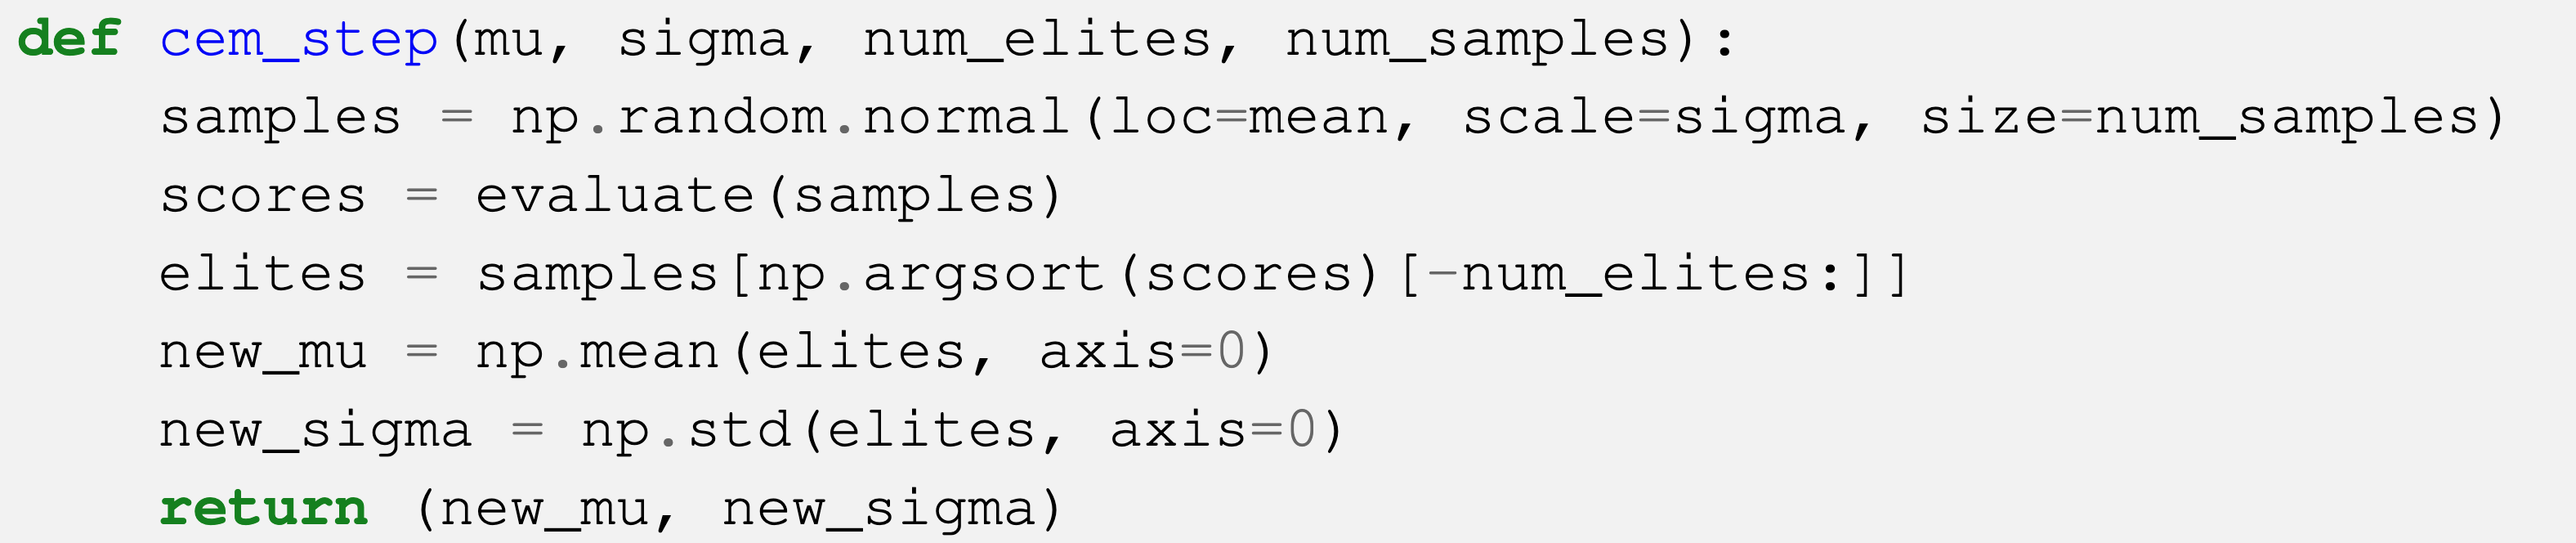
\includegraphics[width=\textwidth]{images/cem_code.png}
    \label{fig:cem_code}
\vspace{-5mm}
\end{figure}

\subsection{\textsc{\implname}}
\label{sec:transformer^2}

The construction of \implname comprises two main steps, for which we provide an illustrative overview in Figure~\ref{fig:method_overview}.
First, we introduce \svdname (\svdacro), a method to learn with RL compact and \textit{compositional} expert vectors based on the SVD of the base model's weights.
Then, we describe three different adaptation strategies within \implname, inspired by three orthogonal principles, which adaptively combine the \svdacro-trained expert vectors during inference.
We motivate how the properties of \svdacro are highly complementary to our adaptation strategies, making \implname an effective and scalable framework for the design of new self-adaptive LLMs.

\begin{figure}[!h]
    \centering
    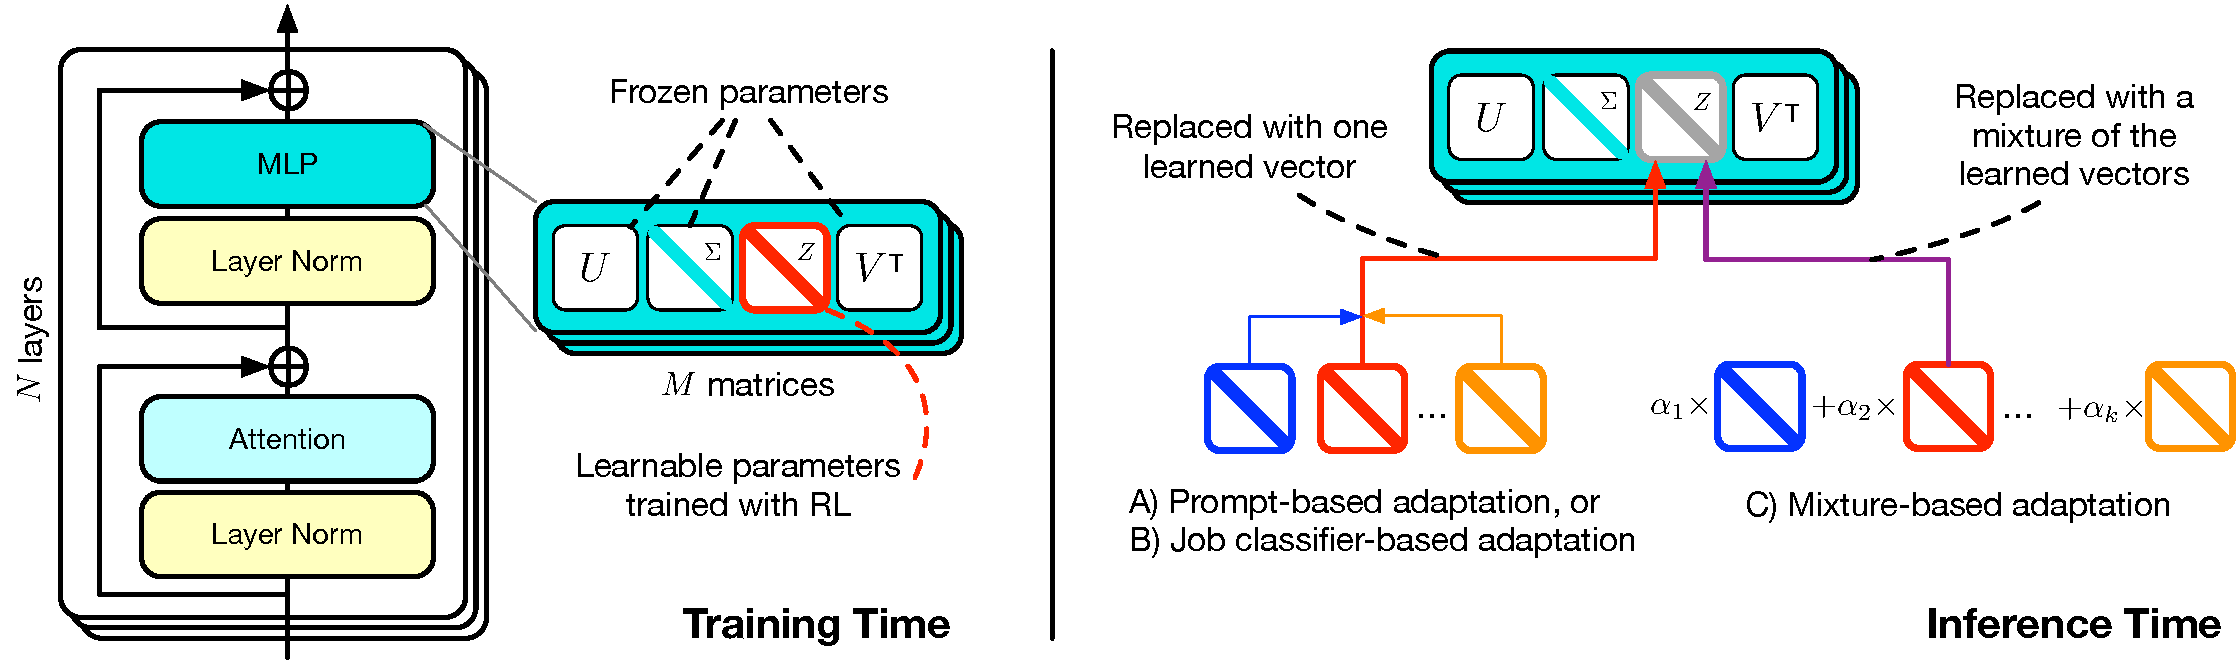
\includegraphics[width=\textwidth]{images/method_overview.pdf}
    % \vspace{-4mm}
    \caption{\textbf{Method overview.}
    Left) At training time, we employ \svdacro and RL to learn the ``expert'' vectors $z$'s that scale the singular values of the weight matrices.
    Right) At inference time, we propose three distinct methods to adaptively select/combine the learned expert vectors.
    }
    % \vspace{-2mm}
    \label{fig:method_overview}
\end{figure}


\textbf{Singular value fine-tuning}\label{sec:svf} is a key building block in \implname.
It offers an extremely efficient parameterization for fine-tuning and provides inherent compositionality for adaptation.
Conventional fine-tuning techniques often aim to augment pre-trained models with new capabilities by modifying their weight matrices.
However, in large-scale transformers,  these weights are already rich repositories of abstracted knowledge, thanks to the breadth of the pre-training data and expansive architectural design.
In fact, as evidenced in much of the prior literature, the requisite capabilities for solving many downstream tasks appear to already exist within these pre-trained models~\citep{sharma2023truth}.
Therefore, instead of seeking to add new features, an efficient fine-tuning approach should focus on making these latent capabilities more expressible. Motivated by these considerations, for any weight matrix $W$, \svdacro learns a simple vector $z\in \mathbb{R}^r$ that provides targeted modifications to each singular component of  $W$ independently, yielding a new weight matrix $W^\prime=U \Sigma^\prime V^\intercal$, where $\Sigma^\prime=\Sigma \otimes\text{diag}(z)$.
This essential parameterization enjoys several benefits:

\textit{Negligible parameters:} Learning only a vector $z$ for each weight matrix allows for very efficient fine-tuning with orders of magnitudes fewer optimized parameters even when compared to prior approaches specifically designed for efficiency. 
For example, the widely popular LoRA approach requires $(m + n) \times r^\prime$ learnable parameters per weight matrix, where $r^\prime$ is a hyper-parameter that generally needs to be set large enough for expressivity. While recent extensions, such LoRA-XS~\citep{balazy2024lora}, try to push efficiency even further, they often introduce limiting assumptions that curb applicability in several practical scenarios (see examples in Appendix~\ref{app:sec:pca}). 
In contrast, while \svdacro only needs $r=\min(m, n)$ parameters, we show it empirically does not display the same shortcomings thanks to working on a highly-meaning space provided by the latent expressiveness compressed in the weights of modern LLMs.
\svdacro's scaling only the singular values may seem to lead to limited expressiveness, we wish to point out that the ability to affect the weight matrix in a full-rank manner technically provides more information than low-rank approaches.

\textit{High compositionality:} Decomposing the weights in independent singular components makes the learned $z$ vectors highly composable and interpretable, opening numerous possibilities for adaptation via algebraic manipulations.
Instead, LoRA-based methods inherently lack these properties. 
For instance, even if two LoRAs learned on the same task were to learn exactly the same adjustments for each $W$, directly interpolating between their compressed $A$ and $B$ matrices is unlikely to preserve any of their original behavior, given the countless number of equivalent parameter permutations they might have converged to.

\textit{Principled regularization:} Exclusively modifying the magnitude of pre-existing singular components provides a principled and effective form of regularization.
In practice, this property enables us to fine-tune for arbitrary downstream tasks with only hundreds of data points without the risk of severe collapse or overfitting.

\textbf{End-to-end optimization with RL.} We train a set of \svdacro vectors $\theta_z = \{z_1, \cdots, z_{N \times M}\}$ to fine-tune an arbitrary language model $\pi_{\theta_W}$ parameterized by $\theta_{W}$ with RL, optimizing directly for task performance.
Here, $\theta_{W}=\{ W_1, \cdots, W_{N \times M} \}$ is the set of weight matrices, where $N$ is the number of layers and $M$ is the number of weight matrices to fine-tune per layer.
We use the seminal REINFORCE algorithm~\citep{williams1992simple} and label each generated answer $y_i$ (for the prompt $x_i\in D$) with a unitary reward based on its correctness $r\in \{-1, 1\}$.
Inspired by related applications of RL for optimizing LLMs~\citep{ouyang2022training}, we regularize the REINFORCE objective by adding a KL penalty for deviating from the original model's behavior, weighted by a small coefficient $\lambda \in \mathbb{R^+}$. Thus, our final objective function can be written as:
\begin{equation}
    J(\theta_z) = \E \left[\log\left(\pi_{\theta_{W^\prime}}(\hat{y}_i \mid x_i)\right)r(\hat{y}_i, y_i)\right] - \lambda D_\mathrm{KL}(\pi_{\theta_{W^\prime}} \| \pi_{\theta_{W}}),
\label{eqn:sec3:reinforce}
\end{equation}
where we use $\pi_{\theta_{W^\prime}}$ to denote the resulting language model after substituting the original weight matrices $W$ with $W^\prime$.
While RL is generally considered less stable than next-token prediction objectives, we find the regularization properties of SVF avoid many of the failure modes of prior less-constrained parameterizations (see Section~\ref{app:sec:ablation_studies}).
Thus, combining these complementary components effectively enables us to avoid relying on expensive fine-tuning procedures with large hand-designed datasets as proxies, and directly maximize task performance end-to-end.

In general, \svdacro with RL puts lower requirement on the dataset it trains on.
For example, LoRA fine-tuning requires ``explaining texts'' to perform next token predictions, which puts a higher requirement on the dataset (e.g., imagine LoRA fine-tuning on a GSM8K dataset where no reasoning text but only the final number is provided).
This benefit allows \svdacro to be more general and effective.
One possible caveat \svdacro can face is the sparse rewards caused by a weak base model, which we discuss this further in Section~\ref{sec:conclusion}.

\textbf{Self-adaptation} is a critical mechanism in nature that has established itself as a core guiding principle in modern system design \citep{7302492}. Our initial efforts toward self-adaptive foundation models focus on the inference stage of LLMs, where we devise a simple two-pass adaptation strategy that combines $K$ sets of base ``expert'' vectors $z^{1:K}$ trained with \svdacro to provide different kinds of capabilities (e.g., coding, math, etc).
The mapping between a capability and the dataset we train on can be acquired in the dataset's meta data.
In the first inference pass, given a task or an individual input prompt, \implname executes the model and observes its test-time behavior to derive a new $z'$ vector tailored to its test-time conditions. 
This adapted $z'$ is then used in the second inference pass to provide an actual response with the newly adapted weights.
The interaction between \svdacro-trained expert vectors and the adaptation strategies ensures seamless integration, where expert vectors provide modular capabilities, and the adaptation strategies dynamically determine and compose the most suitable combination to address the input task.
In this first work, we propose three simple approaches to produce the vector $z'$ during the first inference pass, implementing self-adaption with distinct methods and requirements. Below, we provide an outline of each method and refer to Appendix~\ref{app:sec:implementation} for additional implementation details.


\textit{A) Prompt engineering:}
Our most basic approach involves constructing a new ``adaptation'' prompt which we use to directly \textit{ask} the LLM to categorize the input prompt.
Based on its response, we then extract one category out of the set of domain topics used to pre-train each \svdacro expert and, thus, we select the corresponding $z'$ directly from $z^{1:K}$.
In our adaptation prompt, we also explicitly provide the option for a generic ``others'' category, allowing the model to use its base weights in case no expert provides appropriate capabilities. We show the format used to construct the adaptation prompt in Figure~\ref{fig:sys_prompt}.

\begin{wrapfigure}{r}{0.45\textwidth}
\vspace{-8mm}
\begin{center}
    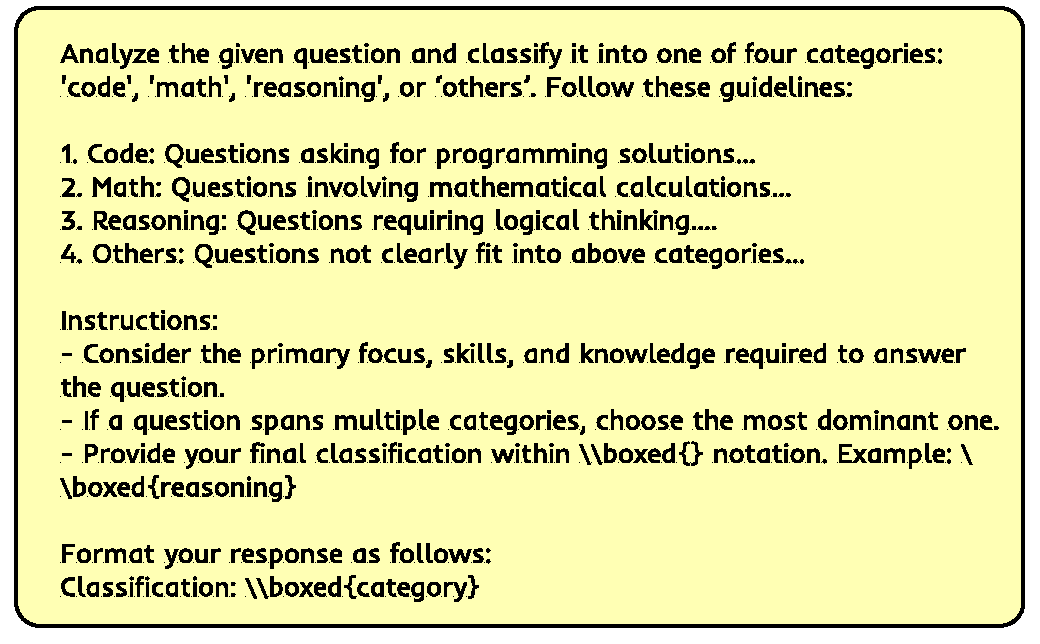
\includegraphics[width=0.45\textwidth]{images/visualization/system_prompt.pdf}
  \end{center}
  \vspace{-5.5mm} 
  \caption{\textbf{Prompt based adaptation.} Self-adaptation prompt used by \implname to classify the task prompt into pre-defined categories.}
  \label{fig:sys_prompt}
  \vspace{-4mm}
\end{wrapfigure}

\textit{B) Classification expert:} 
A direct extension of the prompt engineering approach comes from using a specialized system to handle task identification.
Following the principles of self-adaptation, we apply \svdacro to fine-tune the base LLM itself to handle this task.
In particular, we collect a dataset $D = \{(x_{1,1}, 1), \cdots, (x_{i,k}, k), \cdots \}$ from the $K$ \svdacro training tasks, where $x_{i,k}$ is the $i$-th example from the $k$-th expert task.
Each tuple $(x_{i,k}, k)$ then forms an example to pre-train an additional job classification expert $z^c$ learned in the same fashion as the others.
During the first inference pass, we simply load $z^c$, intending to improve the inherent task classification capabilities of the base model to select a more appropriate $z'$ to handle the input prompt. 

\textit{C) Few-shot adaptation:} Our third approach leverages additional task information by assuming extended access to its test-time conditions beyond individual prompts. 
Our approach is inspired by popular few-shot prompting techniques, which have been shown to provide consistent performance improvements and even allow LLMs to ``in-context'' learn tasks that were entirely unseen prior to inference~\citep{brown2020language}.
For each optimized $W$, our approach entails producing an entirely new $z^\prime=\sum^{K}_{k=1} \alpha_k z_k$ by linearly interpolating between the $K$ learned \svdacro vectors, each weighted by the coefficients $\alpha_k$.
We employ CEM to search over the possible values of each $\alpha_k$ based on the performance on a set of ``few-shot prompts'', which are specifically held out from the rest of the test prompts and used to evaluate CEM's population samples. 
In the case of multiple population samples obtaining the same score on these held-out prompts, we break ties by favoring the one with the highest average log-likelihood across its own generated correct answers.
Crucially, we only need to perform this process once for each target task, avoiding the need to increase the length of each question prompt, a relevant downside of traditional few-shot prompting. We refer to Section~\ref{app:sec:fewshot}, for additional details and an extended discussion of this final approach. 

\vspace{-2mm}